\documentclass[11pt]{article}
\title{Report iteration 2 - SWOP}
\author{Dieter Geboers, Wouter Schaekers, Stefaan Truijen\\ - \\ Professor: Tom Holvoet \\ Project Advisor: Willem Penninckx}
\date{2011-12-31}
\usepackage[pdftex]{graphicx} % fotootjes
\usepackage{fancyhdr} % coole template
\usepackage[top=20mm,bottom=20mm,left=20mm,right=20mm]{geometry} % size and margins
\usepackage{hyperref} % for urls
\usepackage{listings} % code style
\usepackage{textcomp} % voor < en >
\pagestyle{fancy} % ook coole template
\begin{document}
\maketitle

\section{Introduction}
Let's start off by saying we have the feeling that iteration two went a lot better than iteration one.
\\*After the feedback session of iteration one, Thibault decided to drop out of the course. We were left with only three members. We failed to make the deadline for the report on the testing strategy.
\\*However, we did not let that get to us or let it influence the quality of the report, design and code we made. In fact, we put a maximum amount of effort in doing the assignment as best as we could.\newline

Firstly, we will give you a state of affairs and some numbers about the project. Next, we will discuss the big picture from the current software design we made. We'll specifically elaborate on the Scheduler and everything related to it, seeing as we have put the bigger part of our work in creating a scheduler that is very decent. Then we will list some of the "temporary fixes" we implemented, but that we have planned to be improved due to iteration 3. Finally we'll try to draw a couple of conclusions and give you a brief view on our experience of this iteration.
\pagebreak
\tableofcontents
\pagebreak

\section{State of affairs}
We have managed to successfully create a design of every aspect of the assignment. The implementation is almost done, but not just yet. Due to a lack of time(which was probably induced by the fact we hadn't brought iteration one to an end), we were forced to implement a couple of things in a "dirty" kind of fashion. We, however, will implement our actual design by the deadline of iteration three for the following things:
\begin{enumerate}
\item{The way medication items (vitamins, asprin,...) gets handled is currently by using instanceof. We plan to implement a factory pattern here in the future.}
\item{Machines should also be implemented by using a factory pattern instead of "builders".}
\item{Treatments aswell, will be implemented with a factory pattern.}
\item{UnscheduledTaskTest class contains a lot of seemingly random stuff and will be refactored to something cleaner.}
\item{Documentation may be sloppy, missing or inaccurate for some methods and classes.}
\item{Not all methods have been implemented defensively. This is a very small minority of methods. Contrary to iteration one, most methods and classes are completely defensive.}
\end{enumerate}

We have spent an average of 143 hours per person on this iteration. You can find the total amount of working hours for each person in the table below.
\begin{center}
    \begin{tabular}{ | l | l | l | p{100mm} |}
    \hline
    Dieter & Stefaan & Wouter\\ \hline
    115.3h & 167.3h & 149.3h\\
    \hline
    \end{tabular}
\end{center}
For an even more detailed log of the working hours (containing dates and more information about who was present and what happened at what time), we would like to refer to \url{http://code.google.com/p/swop-dswx/wiki/WorkingHours} .

\section{The design}
In this chapter we will inform you about the design we've made and will elaborate on some of choices we have made. Firstly, we have modeled our system in 3 layers. 
\begin{itemize}
\item{User interface layer}
\item{Controller layer}
\item{System layer}
\end{itemize}
All communication from the user with the system has to pass through the layer of controllers (same goes the other way around) to assure that our system does what it is supposed to without getting in an inconsistent state.
\\On the next four pages you will find a class diagram of the system layer of our program. We find this to be the most interesting layer as the controller layer is fairly analogous to what controllers normally look like and as talking about the user interface layer will not inform the reader about what he/she probably would like to know. In order to read the class diagram as it was originally constructed, we would advise you to put the pages next to eachother from left to right. As big class diagrams tend to not be legible, we'd like to refer to an online version of this diagram just in case: \url{http://www.student.kuleuven.be/~s0214045/class%20diagram.png} .\\

\subsection{Patientfilemanager, patientfile, diagnose, treatment}
We had a question about where we should store what treament is associated with what diagnosis. In our eyes, there were two possible solutions.

\subsubsection{Solution}
\underline{Description}: We give PatientFile a field that is a collection of all Diagnosis ever made for this patientfile. Also Diagnosis gets a field that is a collection of all Treatments that have been made for this diagnosis.
\\*\underline{Pro}: Low coupling, high cohesion and information expert for PatientFile are in good shape. PatientFile only has one dependency and does not need to manage treatments on its own.
\\*\underline{Contra}: There will be a deep level of function calls if a list of Treatments is needed: from the controller level all the way over to the Treatment level.
\begin{center}
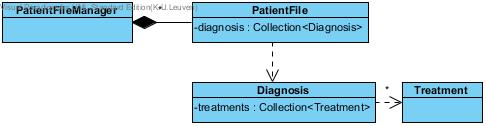
\includegraphics[width=130mm, height=27mm]{patientfilediagwin.jpg}
\end{center}
After a meeting with our project advisor, we noticed that in this solution, the GRASP patterns weren’t violated and the design is arguably elegant. That is why we opted to go with this solution.

\subsubsection{Alternative solution}
\underline{Description}: We keep a map from Diagnose to Treatment in PatientFile.
\\*\underline{Pro}: Easy and efficient access to Treatments.
\\*\underline{Contra}: Gives the patientfile too much responsibility. Also violates the information expert GRASP pattern. 
\begin{center}
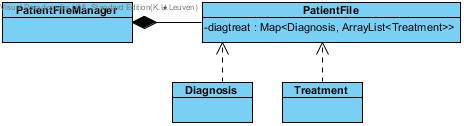
\includegraphics[width=130mm, height=27mm]{patientfilediagfail.jpg}
\end{center}
As stated above, we did not chose to implement this solution after noticing that it violated information expert.\\
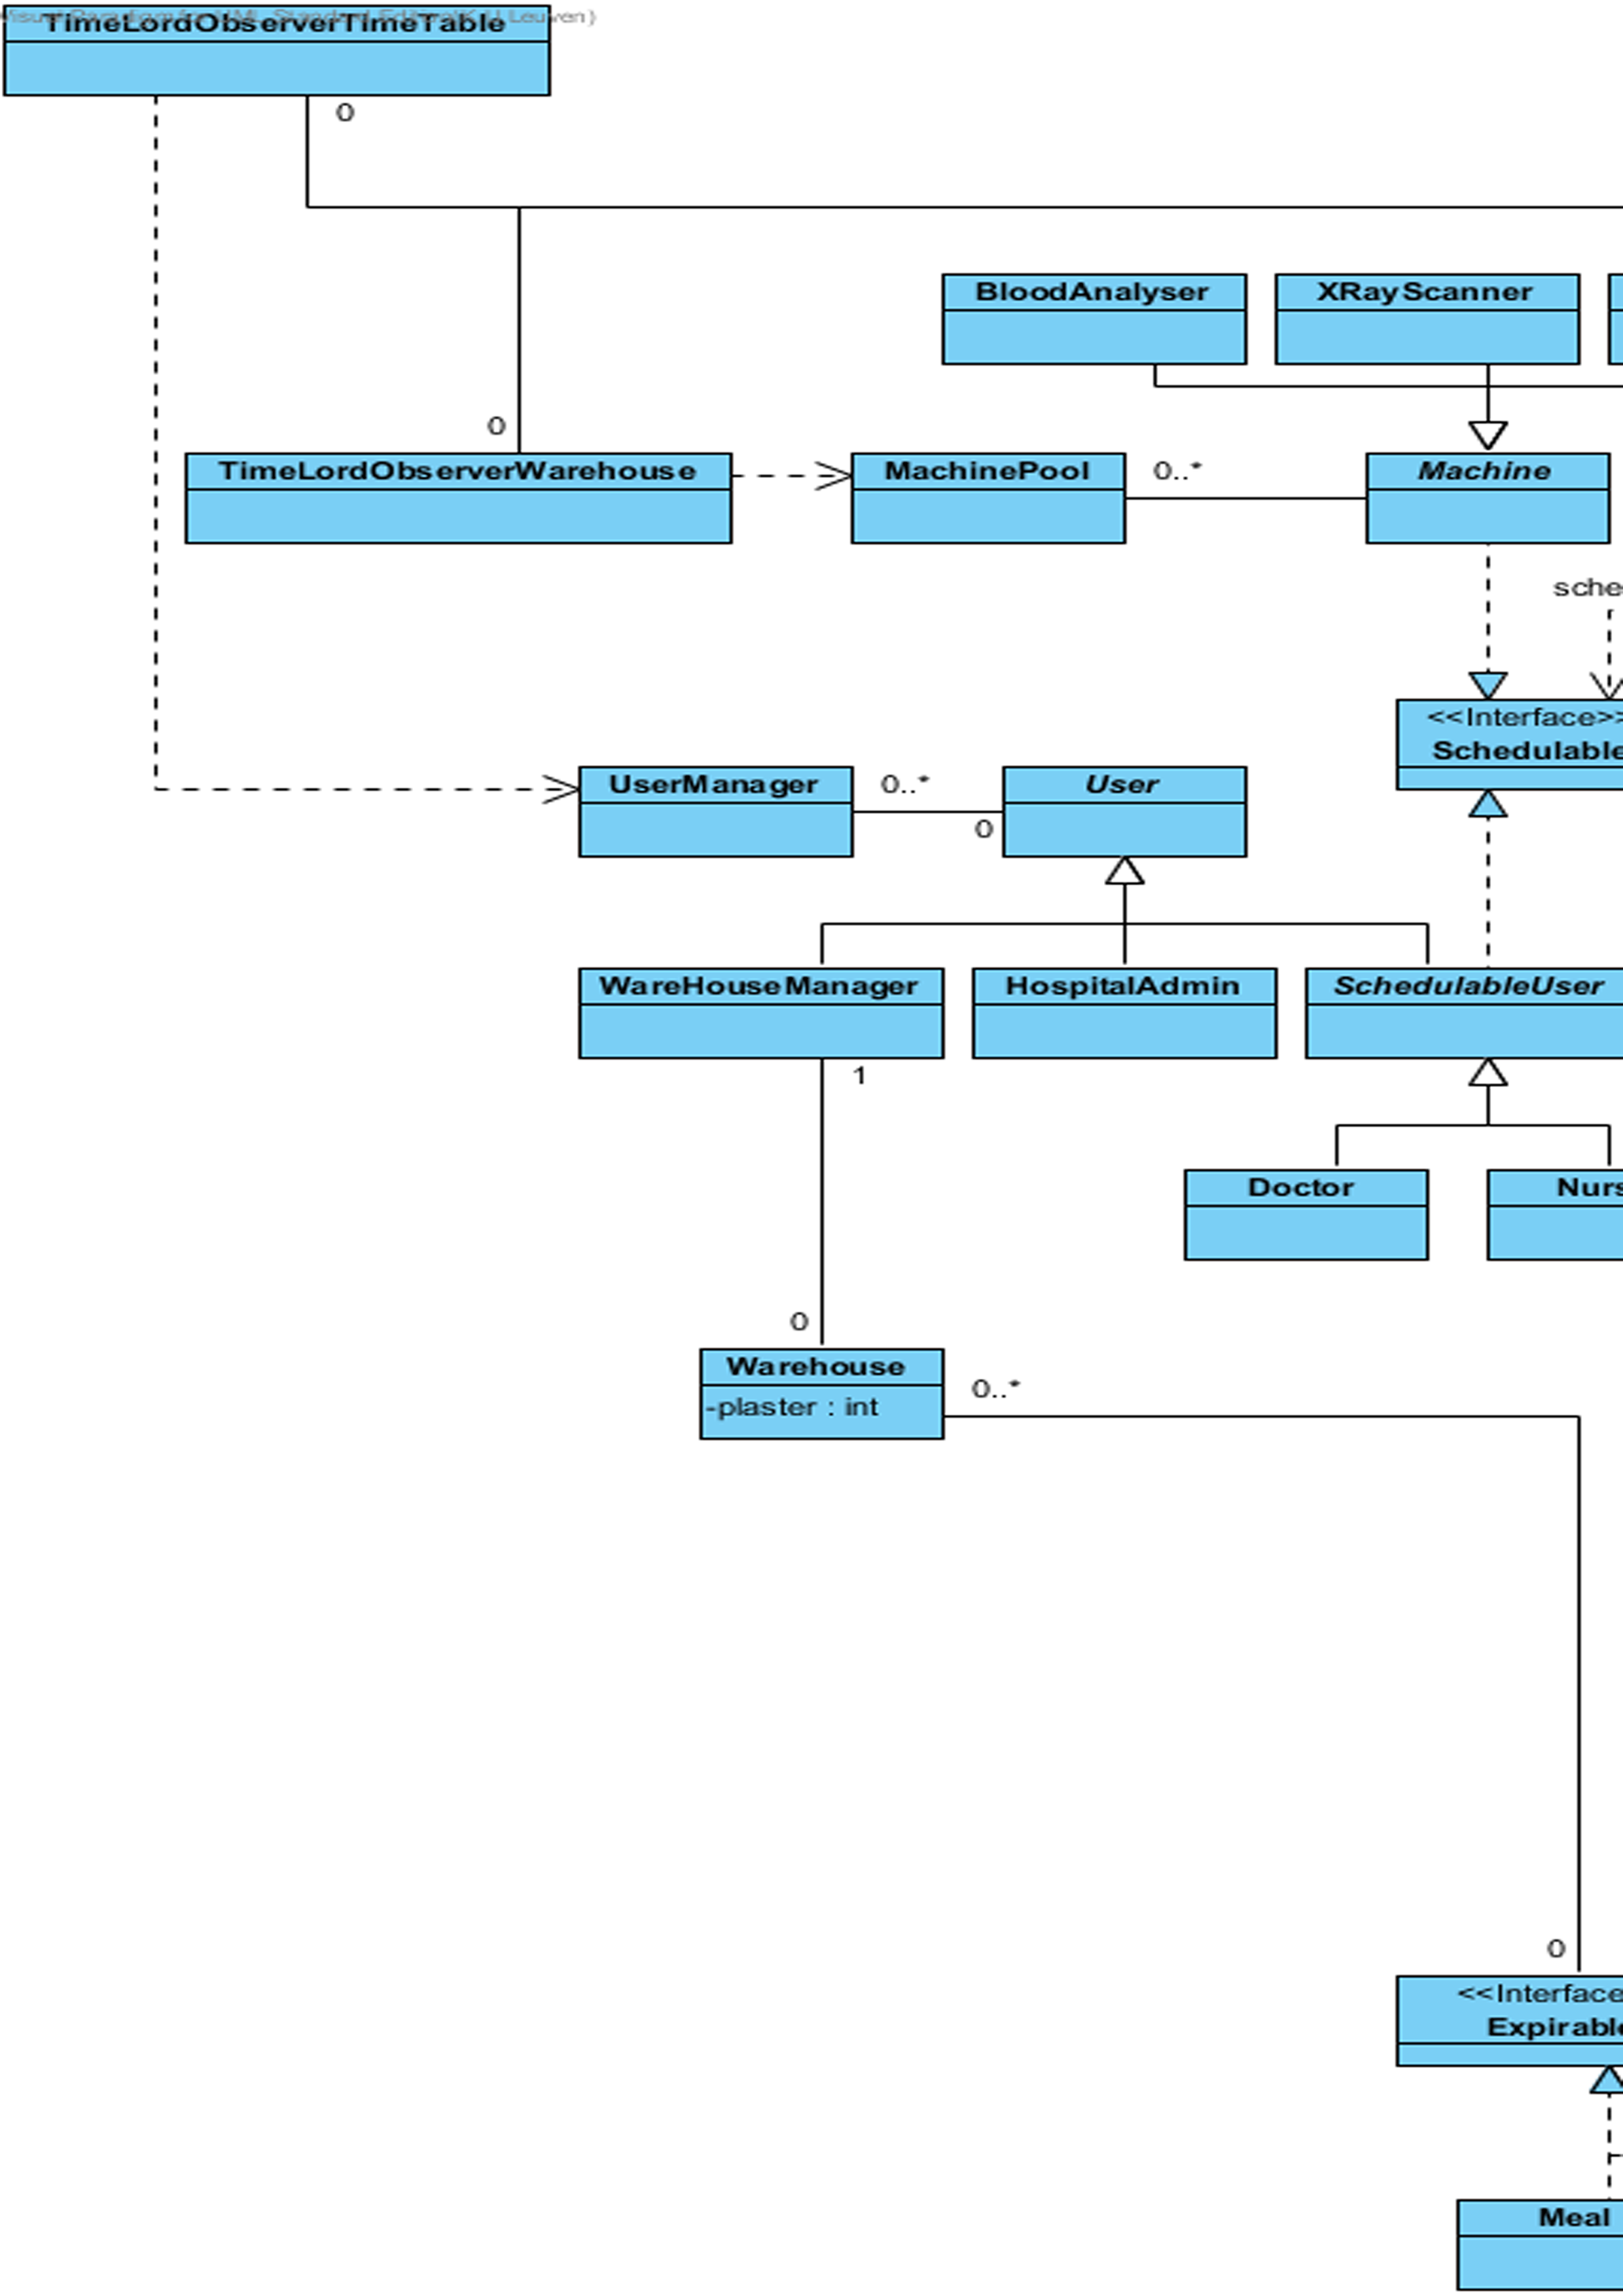
\includegraphics[width=170mm]{left1.png}\\
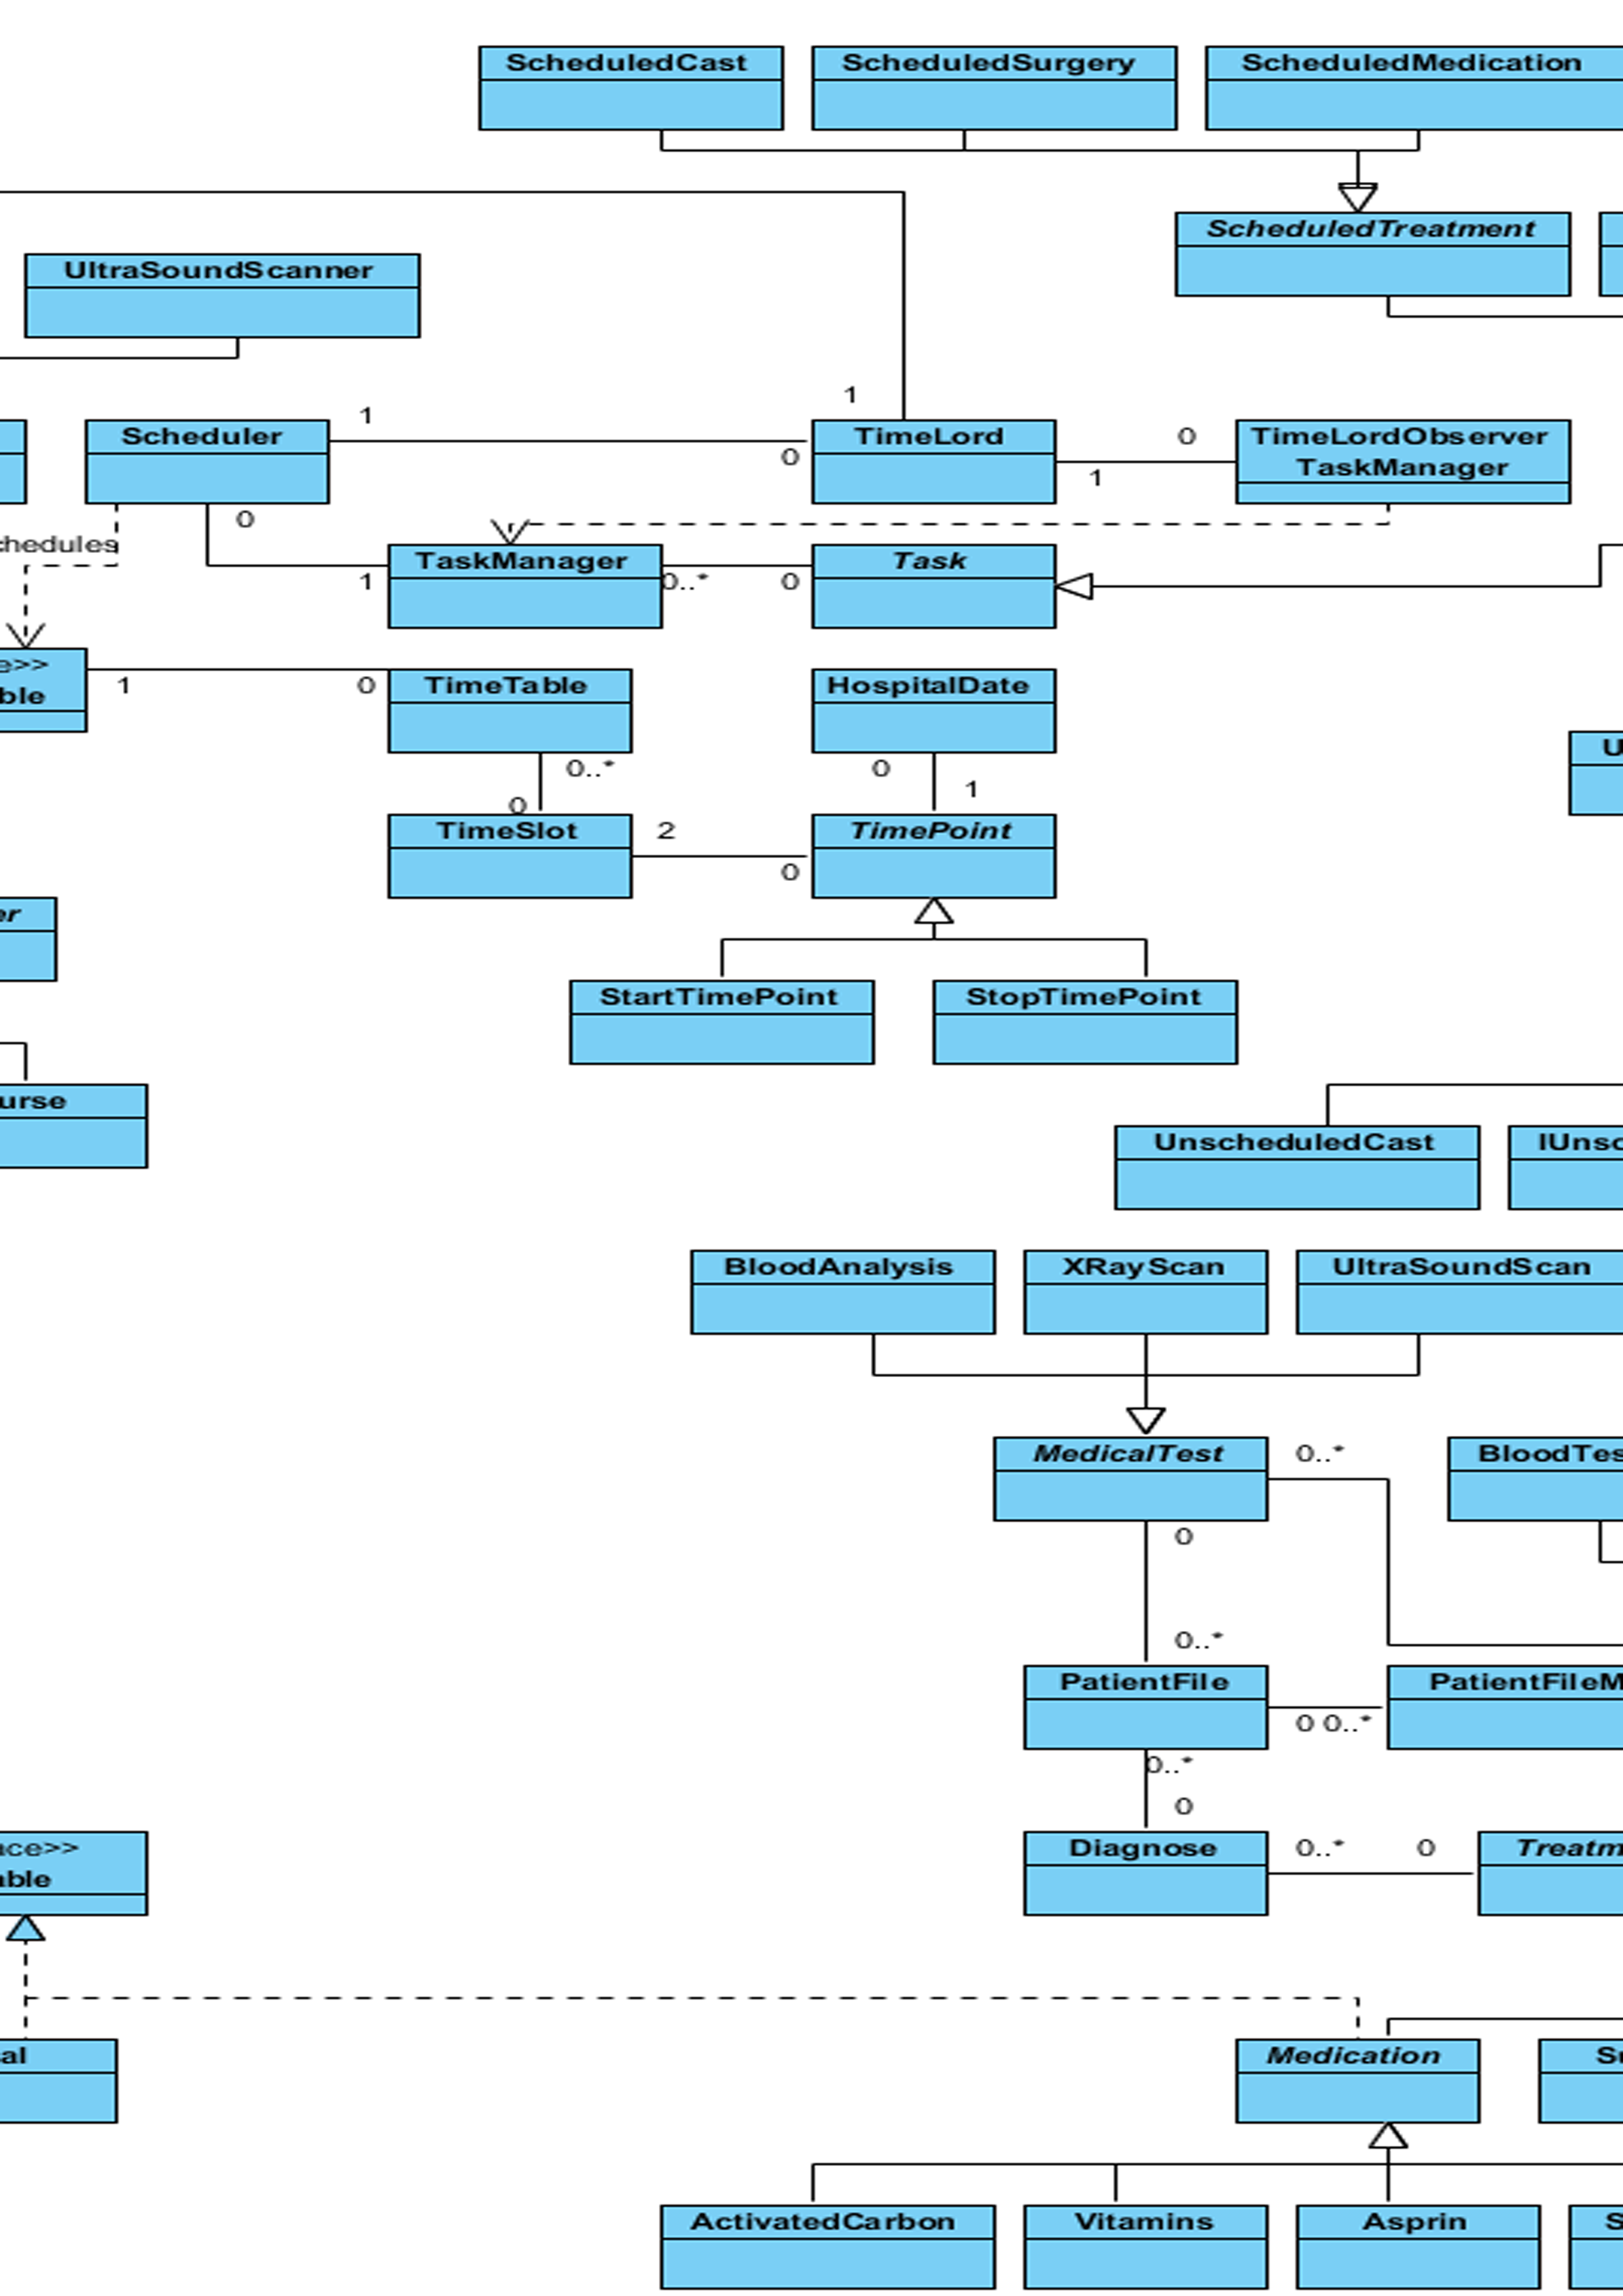
\includegraphics[width=170mm]{left2.png}\\
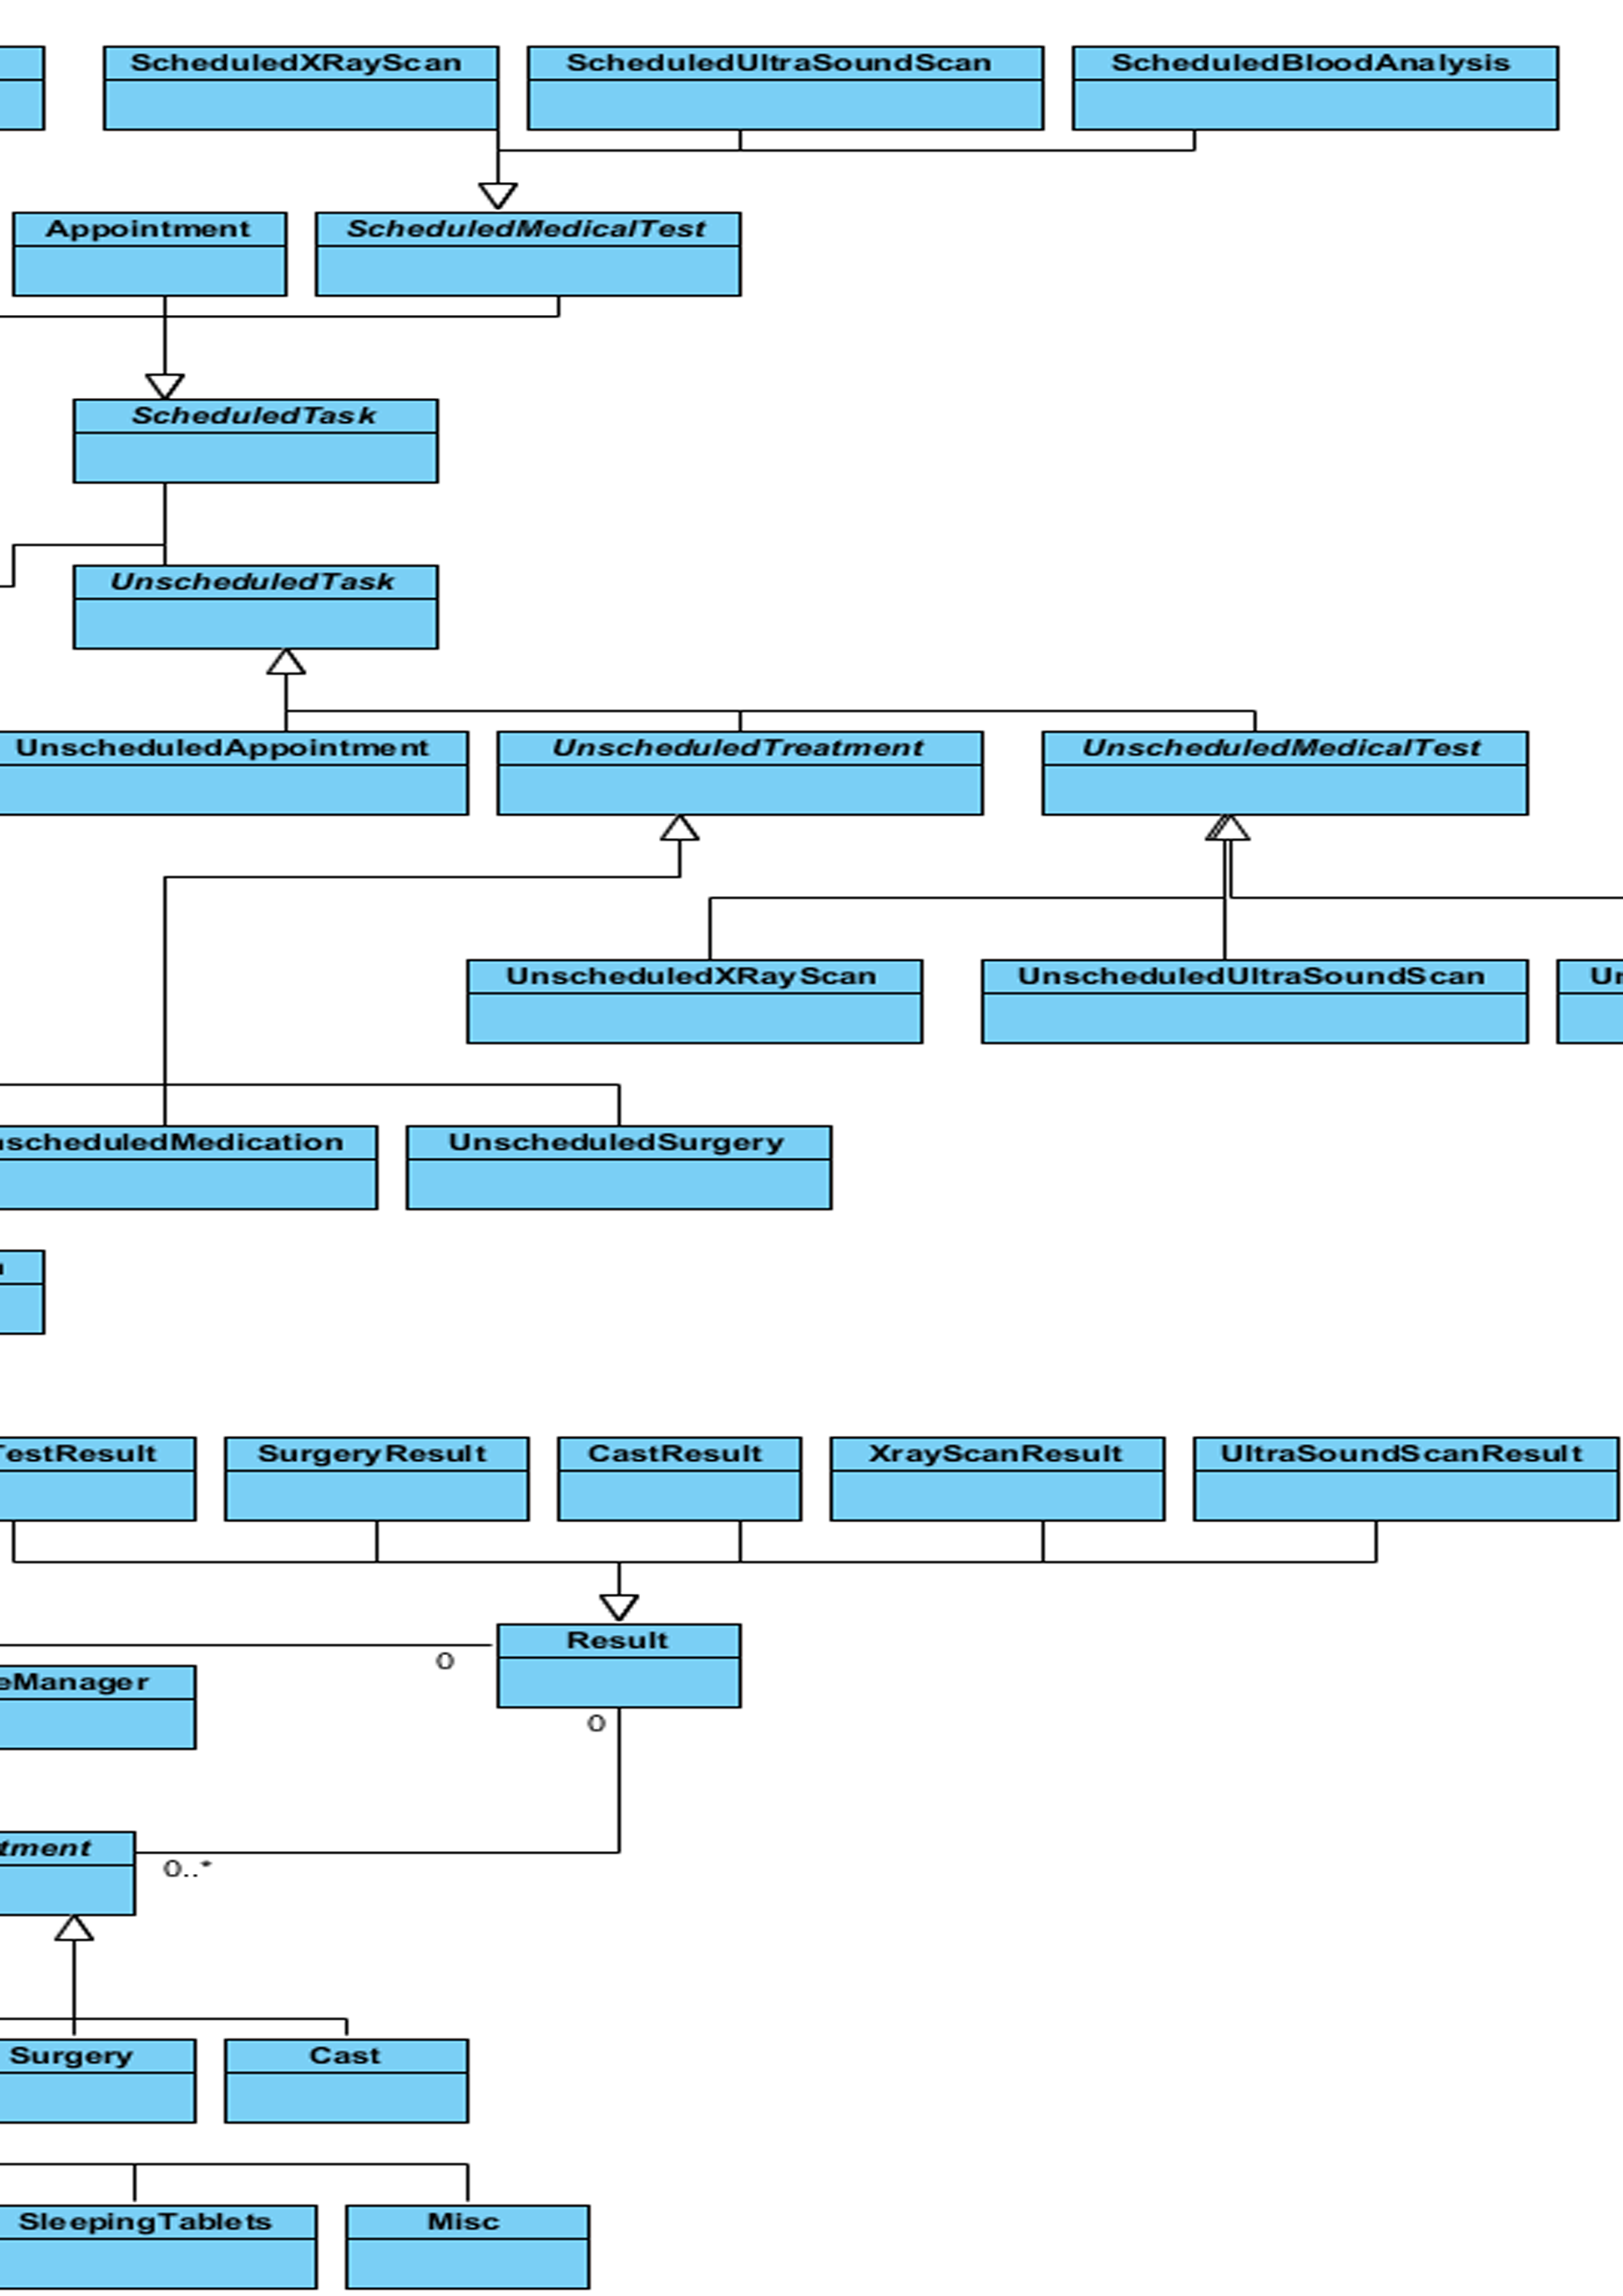
\includegraphics[width=170mm]{middle.png}\\
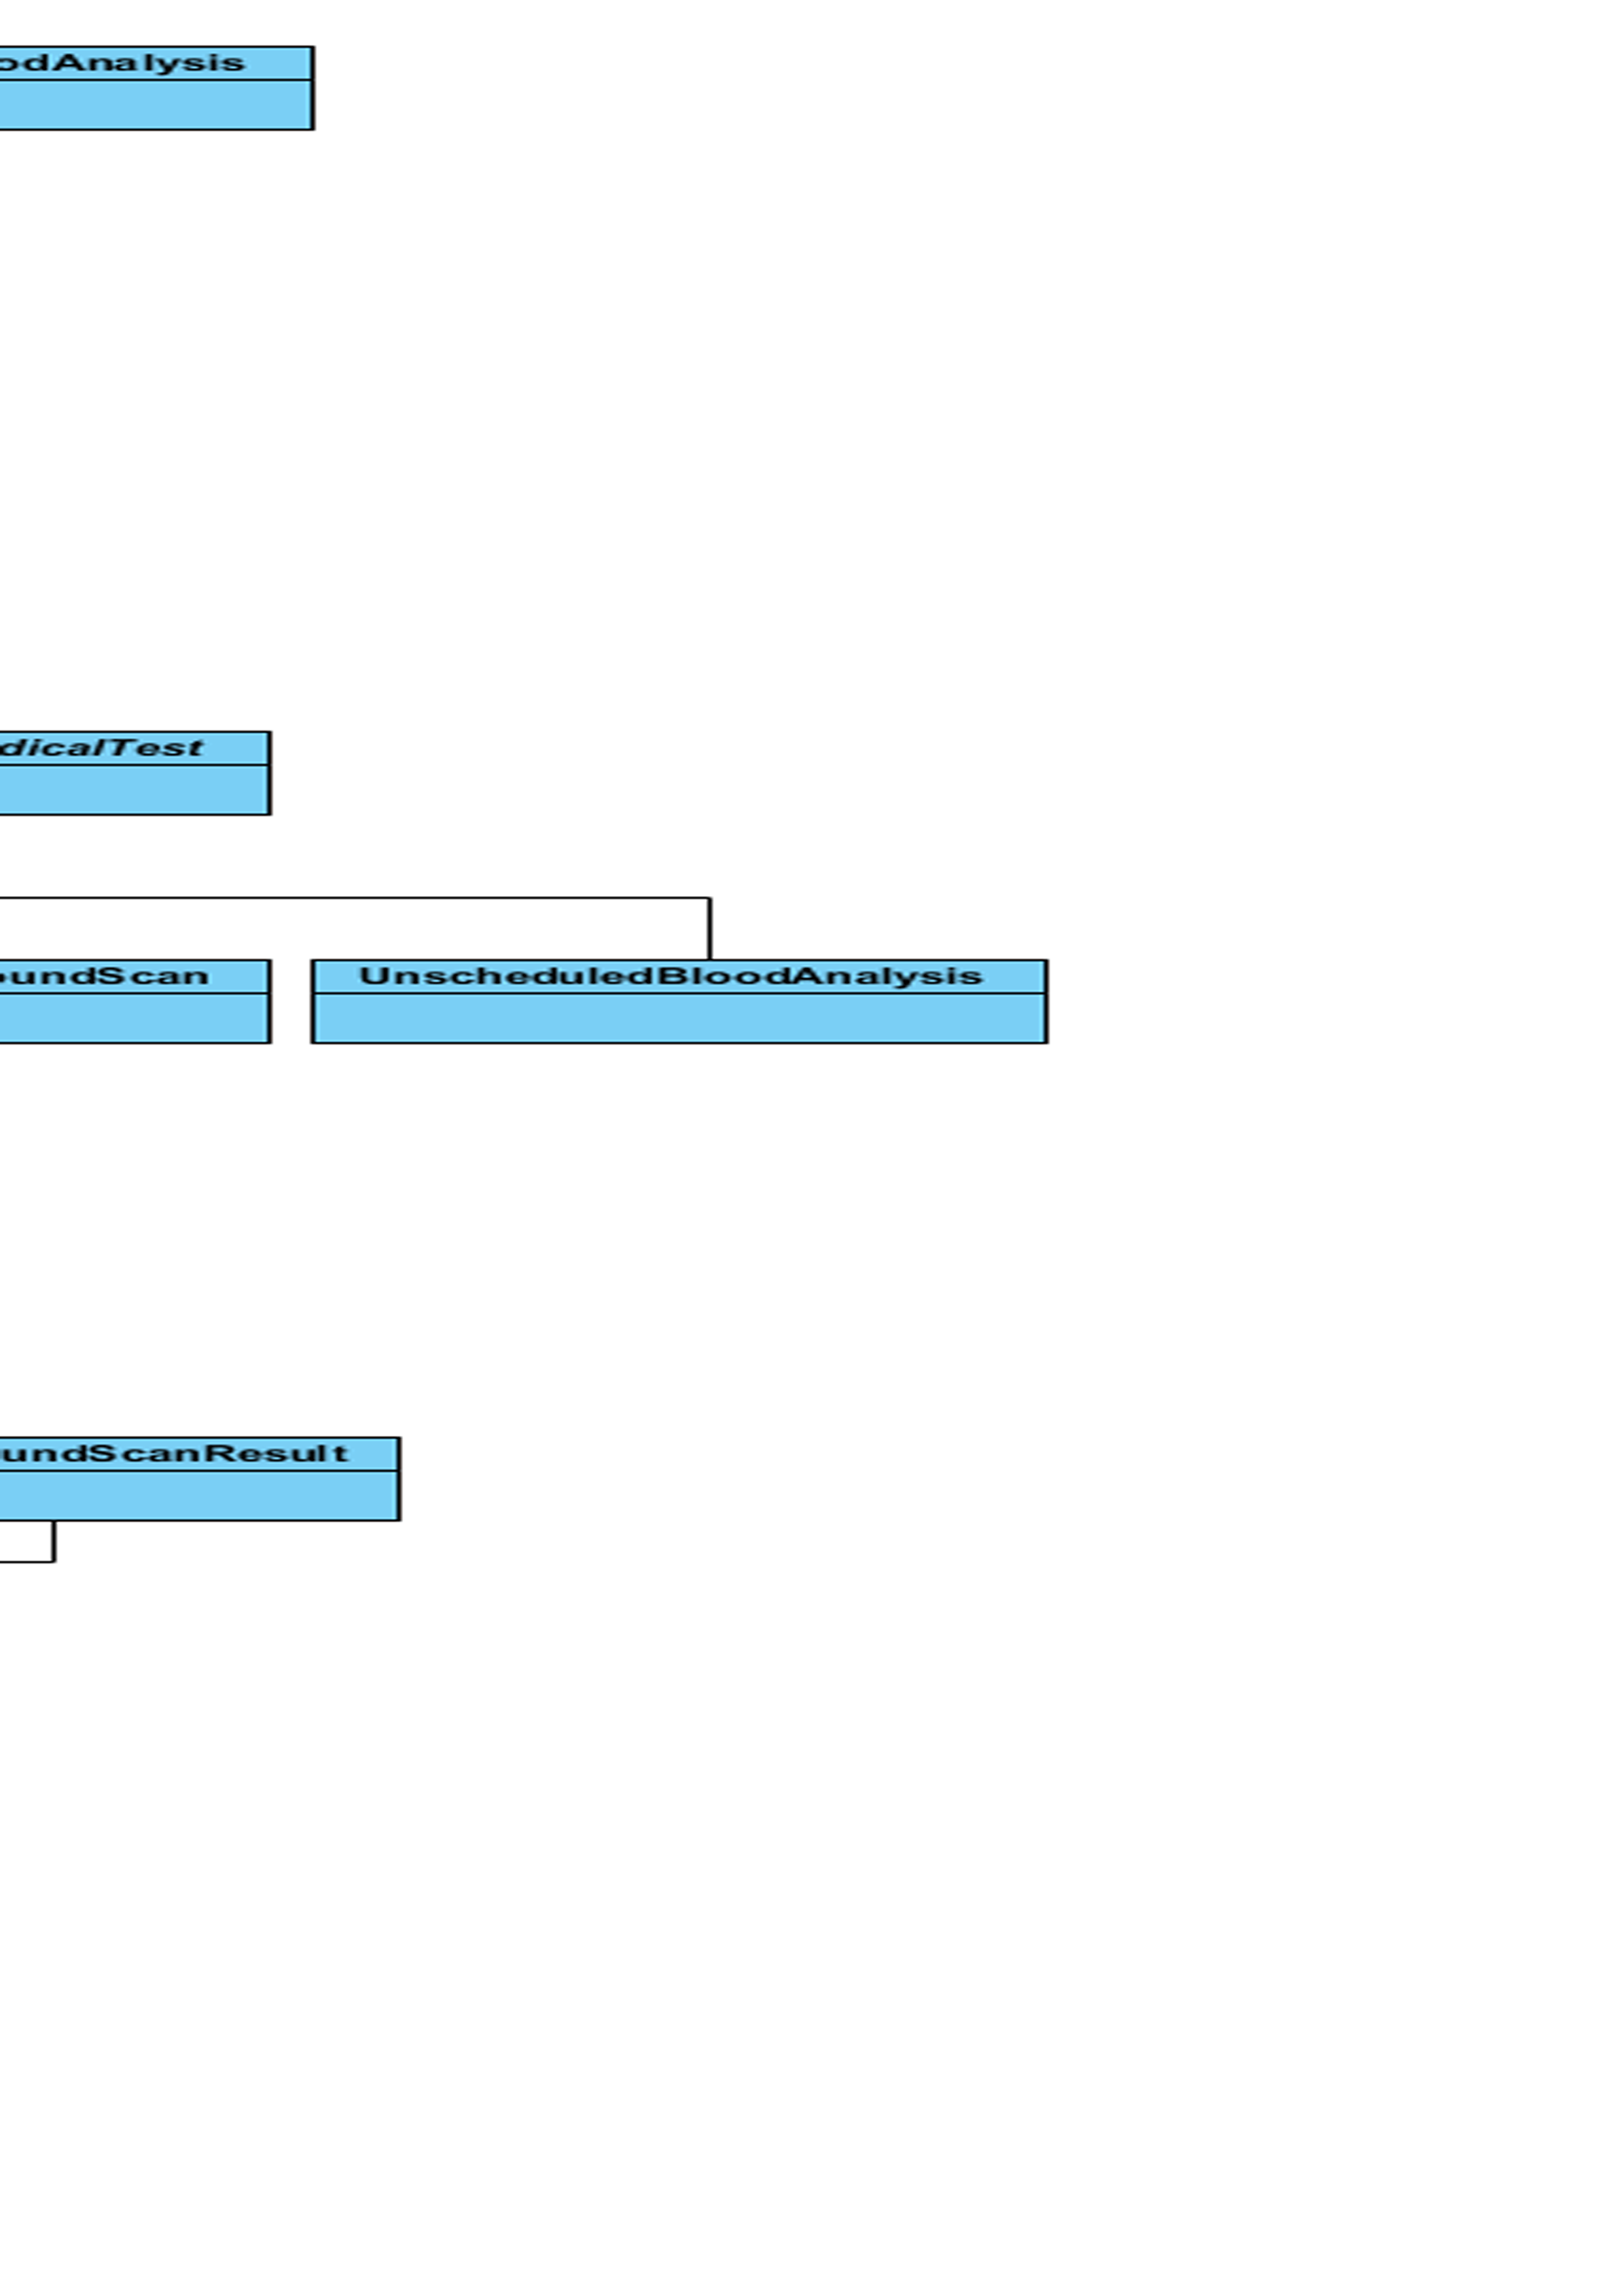
\includegraphics[width=170mm]{right.png}\\

\subsection{MedicalTest, Treatment, Machine and Medication}
While trying to figure out a design that allows us to schedule things in a decent way, we stumbled upon the following problem a couple of times: how can we know at run time what different sorts of MedicalTests, Machines,... there are? The first possible solutions we saw turned out to be outdated after we had a college on design patterns. In the end we decided to implement factory patterns for MedicalTest, Treatment, Machine and Medication. So far, we only found the time to implement the factory pattern for MedicalTest.
\\*The advantages of using a factory pattern is that it's very high cohesion and low coupling; we could very easily remove the factory pattern from the design and still have a relatively stable design. A disadvantage, however, is that, should a new kind of MedicalTest etc... be needed, we'll have to update the class in which all specific factories are stored in aswell as create a new specific factory. We find that the advantages clearly outweigh the disadvantages here, which is why we are very confident about our decision.
\newline Now we'll take a brief look at the alternative solutions we had in mind aswell as their advantages and disadvantages.

\subsubsection{Using enumerations}
\underline{Description}: The idea is that we keep an enumeration for each MedicalTest, Machine,... that's no more than one of a list of final booleans. E.g.: an enumeration for MedicalTest would be:
\begin{lstlisting}
public enum {
	bloodanalysis, xrayscan, ultrasoundscan;
}
\end{lstlisting}
\underline{Advantages}: Easy to implement and understand.
\\*\underline{Disadvantages}: Results in a design with very high coupling. Also written code will not be easily adaptable. The result would be highly similar to using instanceof to determine what kind of MedicalTest a child class of MedicalTest is: unmaintainable. If we would ever need to add or remove a MedicalTest, we would, in this scenario, have to change a very high percentage of code. This means a relatively high chance on accidentally creating bugs. Trying to avoid this would only be possible by keeping a list of all locations in which we have to do something different depending on the type of MedicalTest at hand, which is as exactly silly as it sounds.
\\Clearly, using an enumeration to solve this problem is not a very good way of doing things.

\subsubsection{Mapping Strings onto Objects}
\dots We never really regarded towards this option as a viable solution to the problem. We're just mentioning this to be sure we're giving full and accurate information in the report.
\\*\underline{Description}: This concept is very similar to the enumeration except we'll have all child classes keep a String of their type. E.g. A blood analysis would keep a public final static String containing "BLOODANALYSIS".
\\*\underline{Advantages}: Easy to implement and easy to understand for people just joining in on the project at any time.
\\*\underline{Disadvantages}: Besides the fact that this option is nothing short of a \emph{dirty} hack and not an elegant solution at all, the disadvantages of using an enumeration also return here.
\\*In conclusion: this solution is even more crazy than what it may have looked like in the title.

\subsubsection{Blueprints}
\underline{Description}: This option is interesting to think about. The basic idea is to create templates for different MedicalTests, Machines,\dots. This way, by giving a certain blueprint to a single factory, the factory would create something that meets all the demands of the blueprint. After reading up on design patterns, we see that this solution is a sort of mixture between the prototype and abstract factory design patterns.
\\*\underline{Advantages}: It would be possible, even at run time, to dynamically create new MedicalTests, Machines or even completely new concepts! Low coupling and high cohesion are satisfied in this design. information expert is a bit hazy: blueprints know precisely what they have to, but what about the factory?
\\*\underline{Disadvantages}: The one factory that would turn blueprints into the desired objects, would turn out to be a colosal class with way too much responsibilities and a lot of unclean code.
\\Looks can be deceiving! In spite of this option looking attractive to us at the first sight, we decided that using a real design pattern would probably be better concerning GRASP. Looking back now, we think we have made the right choice.

\subsubsection{Important notes}
It is important to note that not all of the design patterns we want to implement have been implemented yet. Currently the Machine-, Medication- and Treatment problems are still in a sort of hackish state:
\begin{itemize}
\item{In the current version, all types of Machines are stored in a MachinePool. They get created by "\textless machinetype\textgreater builder"s (i.e. "XRayScannerBuilder"). Builders are a softened up version of the factory pattern. We had implemented these builders before we found out about the existence of design patterns and just didn't get to updating it yet.}
\item{The different types of Treatments are also stored in a TreatmentPool. We do not have a builder thing going here. Instead, again due to lack of time, we currently decide what kind of Treatment to create depending on the step of a certain use case that the program is in. For instance, if the user replied they want to create a surgery treatment, we'll create an UnscheduledSurgery. This UnscheduledSurgery becomes a ScheduledSurgery after it's been scheduled. The ScheduledSurgery will keep a Surgery object stored as one of its fields. In this Surgery object, the data about the surgery will be stored.}
\item{As there are different kinds of Medication, there is also need for a cleaner solution than to hardcode what Medication to order in the use cases.}
\end{itemize}
Again, we are aware of these flaws and we plan to get rid of them by the next iteration.
\newline 
The last thing that should be noted is that the constructors from MedicalTest and MedicalTestFactories are only visible within the same package. We opted to do this so as to enforce use of the factories.

\subsection{Scheduler}
We can say with a lot of confidence that we have constantly underestimated the scheduling part of the assignment and everything related to it. Originally we estimated designing and implementing a scheduling system would take about 30\% to 40\% of the total amount of time spent working. It turned out to take over 90\%! It is possible that we went down an exceptionally bumpy road, but we feel it is important we mention this explicitly. 

The idea for the current version of the scheduling solution has been around since early November but only really broke through on December 4th. We dismissed it before that as we did not dig deep enough before judging it. We figured that i.e. nurses keeping their own rosters/schedules was not secure enough and gave the nurses too much responsibility. Later on the idea was refined a little bit more. During the refining process it quickly became clear that the choice to have TimeTables for each Schedulable was way better than any of the other scheduling propositions we had come up with.

If you look back at the four page class diagram, you'll notice a reasonable scheduling design. Let's take a closer look right away and explain what some classes are for. After discussing those classes, we'll list some scheduling versions we also have spent a notable amount of working time on with their advantages and disadvantages compared to the current design.

\subsubsection{HospitalDate}
We had started implementing the system that’s in the class diagram above by using java.util.Date. We soon found out that there was something not right with this library. The methods used to get the year, date, hour,… of a Date-object are all depricated and do not work at all in combination with the not-depricated constructor and toString() of Date. After numerous frustrations about Date, we considered a number of possible alternatives.
\\The most evident alternative would be java.sql.Date. However, this library does not vary all that much from java.util.Date and we found it just almost just as dysfunctional as the latter. The next possible solution was to work with Calendar objects from java.util.Calendar. Unfortunately using this class is not as programmer friendly as one would expect it to be. We would like to quote Joshua Bloch, Google's chief Java architect and author of “Effective Java”, from an interview in which he was asked to give some tips for Java developers. In this interview, he said the following:
\begin{center}
\emph{"As an extreme example of what not to do, consider the case of java.util.Calendar. Very few people understand its state-space -- I certainly don't -- and it's been a constant source of bugs for years." - \url{http://java.sun.com/developer/technicalArticles/Interviews/bloch_effective_08_qa.html} .}
\end{center}
We then opted to go with java.util.GregorianCalendar instead. While a significant improvement over Calendar, GregorianCalendar still proved to be rather hard to work with. Finally we decided to write our own Date class and named it HospitalDate. This class uses the GregorianCalendar to store and calculate dates, but we implemented some getters and setters so that using a HospitalDate would make our code easier to read and write. HospitalDate turned out to be exactly what we needed as it did not have any of the disadvantages of the other alternatives mentioned above.
\newline HospitalDates have a constructor that allows you to create a Date that takes place at a certain amount of milliseconds since the system start time (8AM at Nov 8th, 2011): the so called "start of time". "End of time" is the point at which the value of long would overflow, if added one more millisecond. All methods returning milliseconds or asking milliseconds as a parameter work in this way. 

\subsubsection{TimeTable}
A TimeTable is a class that represents the individual TimeTable that each Schedulable has. It very much resembles a real life timetable in which one can keep track of one’s appointments and todos. A TimeTable consists of a set of TimeSlots. Each TimeSlot in the TimeTable represents an interval in time during which the TimeTable in question is marked as being “occupied”. A couple of methods in TimeTable that are worth mentioning (as they're not in the class diagram):
\begin{itemize}
\item{invert() : TimeTable}
\item{getUnion(TimeTable) : TimeTable}
\item{getIntersect(TimeTable) : TimeTable}
\item{eliminateOverlap() : void}
\end{itemize}
Invert() inverts the TimeTable. This means: busy slots become free slots and the other way around. The result of this method is a new TimeTable that is the inverted one of this TimeTable. Evidently the inverted TimeTable of the inverted TimeTable of an original TimeTable, is the original TimeTable again. This method can be very useful to determine all free slots in a  TimeTable. 
\\*getUnion() gets the union of two TimeTables. The union is defined analogous to the union of two collections in mathematics: it’s a new TimeTable that is marked as “busy” everywhere where either one or both of the original TimeTables is “busy”.
\\*getIntersect() gets the intersection of two TimeTables. Like getUnion(), getIntersect() is defined very much like in mathematics: the intersection of two TimeTables is a new TimeTable that is marked as “busy” where both of the original TimeTables are “busy”.
\\*eliminateOverlap() is a method that basically merges timeslots that overlap. For example: if a TimeTable contains a slot from 5AM to 8AM and another one from 7AM to 9AM, eliminateOverlap() will result the two original timeslots being reduced to only one: from 5AM to 9AM.

\subsubsection{TimeSlot}
A TimeSlot is nothing more than a representation of an interval of time. It has a starting- and stopping point. Its length is in milliseconds.

\subsubsection{TimePoint}
As a TimeSlot has a starting and stopping point, TimePoint is the abstract class that represents those points in time. Each TimePoint has a HospitalDate so as to know which point in time it really represents.
\\*It has two child classes: StartTimePoint and StopTimePoint. At first TimePoint held on to an enumeration so that it would know whether it was a starting- or stopping point. Now however, the design is more adaptable: it's easily possible to add a new sort of TimePoint now due to the high cohesion achieved by using two separate classes.

\subsubsection{Schedulable and SchedulableUser}
Schedulable is an interface that is implemented by all objects that can be scheduled in the hospital (i.e.: nurses, doctors, XRay scanners, bloodanalysismachines,…). Because hospital administrators and warehouse administrators can’t be scheduled for now, there is also a distinction between User and SchedulableUser, as you can see in the class diagram.
Schedulable objects have three methods worth mentioning: 
\begin{itemize}
\item{canBeScheduledOn(HospitalDate startDate, HospitalDate stopDate) : boolean}
\item{getTimeTable() : TimeTable}
\item{scheduleAt(TimeSlot timeslot): void}
\end{itemize}
These methods should do what their names suggest they do. canBeScheduledOn() will return true if the object executing the method finds that all it’s privately kept constraints have been met and that its TimeTable allows it to be scheduled at the given interval of time. getTimeTable() will get and return the TimeTable of the Schedulable in question. scheduleAt() will schedule the Schedulable at the given TimeSlot if possible.

\subsubsection{Constraints}
There are a lot of constraints related to time and scheduling in this assignment. I.e.: nurses only work between 8AM and 5PM, Treatments can be registered before being scheduled, everything must be scheduled at least 1 hour in advance of the current system time, a patient may only get ten XRay scans per year,\dots. Most of these constraints can be taken care of by either canBeScheduled() in Schedulable, or the use case. As there are use cases, we can be assume some things are given for the implementation of several functions in the system layer of our model.
\\*A constraint that has risen a problem was the fact that a Diagnose can already have a Treatment without it being scheduled, if the Diagnose is not approved yet at the time of the creation of the Treatment. We'll elaborate on this in the sections below.

\subsubsection{Task, UnscheduledTask, ScheduledTask, TaskManager}
Task, UnscheduledTask and ScheduledTask are all abstract classes that represent things that can be (or already have been) scheduled. UnscheduledTasks are Tasks that haven't been scheduled yet. Once they can be successfully scheduled by Scheduler, they can be removed from the taskqueue kept by TaskManager and turned into ScheduledTasks. The ScheduledTasks get stored in the resources that are to execute the ScheduledTask so that giving the user sensible output concerning todos is almost trivial.
\\* As is, it is possible a Task can't be immediately scheduled after creation. Possible reasons for this could be: the warehouse has run out of stock of an item required by the Task just recently created or the Task that can't be scheduled is a Treatment for a Diagnose that has not been approved yet. We managed to solve both of those problems by implementing the observer pattern. We now have a couple of Observers that get notified at the right times and that then tell the TaskManager to update its queue as some changes in the system has triggered the observer watching it.

\subsubsection{TimeLord}
TimeLord is the class that keeps track of the current system time. We have chosen to create a seperate class for that purpose only. The alternative was to keep the current system time stored in Scheduler. However, we felt like this does not fall under the responsibilities of Scheduler. 
\\*Let's assume one would like to keep the current system time in Scheduler. They then would have to make a choice between having the system time be static or not. A static system time is bad for the following reason: any class extending scheduler will not be able to keep their own system time should another scheduler or sub class of Scheduler already exists. Expanding the hospital into several timezones or creating a new sort of Scheduler, would then not be possible. The only option left then is to keep it as a non-static field. That would mean that any class requiring the system time would depend on Scheduler. This is bad for low coupling and high cohesion as a very high amount of classes will then depend on the Scheduler.

\subsubsection{Observers}
TimeLord also has four Observers in case the current system time should change. One of them notifies the warehouse, another the TaskManager, yet another one the Schedulables and the last one the StockManager. The first Observer will trigger the expired medication in the warehouse to be removed aswell as the meals to be eaten (if needed). The second one will trigger an update of the task queue. The third one will get the Schedulables to remove their ScheduledTasks if they have already been carried out and the last one will notify the StockManager to update the StockOrders.
\\*Warehouse also has two observers. One of them notifies the TaskManager and the other one the StockManager. The reason for this is quite logical: if the warehouse contents change, then that means that there either was more stock delivered or that there are items that have been removed due to a scheduling call or removal of expired items. If more stock has been added, then it is possible that some UnscheduledTasks from the task queue in TaskManager suddenly can be scheduled (e.g. they couldn't be scheduled immediately as there was not enough plaster, but then plaster gets added. If that's the case, then they CAN be scheduled). If stock was removed, then it is possible that the hospital finds that there is not enough stock left for the near future. This triggers an Observer to report that the contents of the warehouse have been changed to the StockManager.
\\*Last, but not least, there's an Observer for Diagnose. It reports changes to the validity of a Diagnose to TaskManager. Again the reason is quite logical: should a Treatment not be able to be scheduled immediatly after creation, then either there wasn't enough stock left to carry out the treatment or the diagnose for which the treatment was described wasn't approved yet at that time. If it's the latter, then a change in the validity of the diagnose will trigger the Treatment to be scheduled by TaskManager via the Observer.

\subsection{Alternatives for the scheduling problem}
We have ran quite a lot of alternative designs for the Scheduling problem by eachother and our project advisor over the past 3 months. We will now briefly discuss what some of them were and what their advantages and disadvantages were. It should then be absolutely clear (if it wasn't already ;-) ) why our current Scheduler is the better one.

\subsubsection{Original version}
The original version of the solution to the scheduling problem was one that "just works". It violated almost every one of the GRASP patterns: it did all the constraint processing, it depended on almost every other class, it kept the current system time, it kept the schedule of EVERY individual Schedulable stored in a TreeMap and had quite lengthy methods that, to an outsider, may seem almost magical.
\\*There were no advantages of this design. It just worked but had so many disadvantages that it took a long time before we turned it into something less gruesome.

\subsubsection{First revision}
The first revision we made was a form of patch for the original Scheduler. We removed constraint processing from the Scheduler class and added a couple of new classes: Task, ASpecificResourceRequirement, ANurseRequirement, TaskManager, ScheduledElement,\dots You can find a class diagram of this design in appendix I.\\
We removed some of the responsibilities of Scheduler and moved them to Task. This still violated the information expert aspect of the GRASP patterns, but it was less bad as the original version.

\subsubsection{Second revision}
The next revision contained a ConstraintProcessor and Constraint class for constraint processing purposes. This does satisfy the GRASP pattern that has been violated in the previous versions more, but implementation of ConstraintProcessing led us too much towards reinventing Prolog. For the class diagram of this revision, please see appendix II.

\subsubsection{Third revision}
In this revision we created TimeTables, TimePoints, TimeSlots, Schedulable, TaskManager and got its responsiblities straight. It's the base of the current version.  This version had as advantages that it had object-oriented design, was straight forward and logical. However, there were still enums present at several locations. UnscheduledTask and ScheduledTask also turned out to be too generic for the purposes we wanted them to serve. We attempted to update the flaws of this revision in the current revision. You can find a class diagram of this revision in appendix III.

\section{Use cases}
The following use cases have been implemented (not all have been debugged though!):
\begin{enumerate}
\item{Login}
\item{Logout}
\item{Register patient}
\item{Order medical test}
\item{Add hospital equipment}
\item{Add staff}
\item{Advance time}
\item{Enter diagnose}
\item{Approve diagnose}
\item{Consult patientfile}
\item{Review patientfile}
\item{Discharge patient}
\item{Close patientfile}
\item{List orders}
\end{enumerate}
That leaves us with the following usecases left to implement:
\begin{enumerate}
\item{Enter result from medical test}
\item{Enter result from treatment}
\item{Prescribe treatment}
\end{enumerate}
We implemented the use cases in the same way we implemented them for the first iteration. However, our explaination may have not been as good as it should have been. We will thus attempt to rephrase and explain again how our use cases work.
\\*The user interface is based on both the Command pattern and the State pattern. All the states implement the following interface:
\begin{lstlisting}
interface state
{
   public state execute();
}
\end{lstlisting}

\begin{lstlisting}
while( currentState != null )
    {
        currentState = currentState.execute();
    }
\end{lstlisting}
An example of how this works is given in the following piece of code, it queries a user for his or her name and if the name has less then 4 characters the name will be queried again.
\begin{lstlisting}
class MainMenu extends state
{
    state[] menu_options = new state[1];
    public MainMenu()
    {
       state[0]=new AskName();
       state[1]=null;
    }
    
    public state execute()
    {
        print("Select the menu option you want to take");
        print("Option 1, input name");
        print("Option 2, quit");
        int i = readInteger();// error checking ommited for breverity
        return menu_options[i];
    }
}

class AskName extends state
{
    public state execute()
    {
        print("Enter your name: (more then 4 letters)");
        string name = readLine();
        return new CheckForValidName(name);
    }
}

class CheckForValidName extends state
{
    string name;
    public CheckForValidName(string name)
    {
        this.name=name;
    }

    public stat execute(){
        if(validName(name))
        {
            return new NameSuccesfullyEntered(name);
        }    
        else
        {
            print("invalid name please enter new name");
            return new AskName(); 
        }
    }

    private boolean validName(string name){
    if(!validLength(name))
        return false;
    return true;
    }
    private boolean validLength(String name)
    {
        if(name.length() < 4)
            return false;
      return true;
  }
}
class NameSuccesfllyEntered 
// omitted for breverity
\end{lstlisting}
Advantages of this approach are:
\begin{itemize}
\item{UI is easy to debug and write;}
\item{UI has a clear flow and every state has it's own use;}
\item{The user interface is well structured.}
\end{itemize}
While we keep the following disadvantages in mind:
\begin{itemize}
\item{User interface will have a very large amount of classes;}
\item{This approach is not that obvious to understand;}
\item{State transitioning diagrams are practically required to follow the state transitions.}
\end{itemize}

\section{Other notable changes}
Aside from the design choices we mentioned above, there were some other notable smaller changes this iteration that we will briefly discuss next.

\subsection{No more enumerations!}
We were able to get rid of all enumerations and thus achieve a higher grade of adaptibility.

\subsection{Domain protection - not leaking internal data structures}
Instead of leaking internal data structures, as was the case in iteration one, we now have made sure that all methods return a safe copy when needed. We achieved this by implementing read-only objects as interfaces that only have methods that other classes should be able to access. e.g.: NurseIN is the interface to which a Nurse can be cast to before returning her to another class or model layer.
\\Also methods that returned pointers to field where they shouldn't now return either deep copies or clones.

\subsection{Defensive programming}
We have tried our best to make all classes from the system layer as defensive as possible, only catching exceptions in the user interface layer. We have some doubts about throwing some exceptions in constructors of certain classes though; i.e. new Diagnose() throws InvalidTimeSlotException does not seem very correct\dots

\section{Eclemma testing report}
Currently the total amount of lines of code has passed 20,000 with over 260 classes! Of those ~21,000 lines, Eclemma tells us that 108 unit tests cover 43.3\% of the code. 
\\*About 4,600 lines of those are use cases. We opted not run tests for the UI packages with unit tests as the results depend on user input, which is harder to program than to just debug them with trial and error. That puts us, without the use cases taken into account, on about 55\% code coverage.

\section{Todos for next iteration}
As mentioned in the report there are still some things that aren't completely done yet. There are some use cases left to implement, we should realise factory patterns where there are some temporary dirty solutions for now (MedicalTest, Machine,...). We'll need to create Observers for MachinePool and UserManager, as for now there's still a small problem in the following situation:
\\Suppose you have a hospital without ultrasound scanners. Create a UnscheduledMedicalTestTask that requires an UltraSoundScanner. This Task will be put in the task queue of TaskManager as it can't be scheduled right away after creation. Now we have the hospital administrator add a new UltraSoundScanner. The previously created Task will not be scheduled until any of the already existing Observers of TaskManager get notified. To solve this, an Observer for MachinePool and an Observer for UserManager should suffice.

Currently there are 4 classes for every 1 kind of MedicalTest and 4 classes for every 1 kind of Treatment (the test itself, the unscheduled task, the scheduled task and the result). We should develop a more clean design for those. We're currently thinking we could do something with a State pattern.

The amount of code coverage was also rather low. We will have to write more unit tests during the next iteration.

\section{Conclusion}
We have worked as best we could to make up for the failure of iteration one in this iteration. We have achieved a lot but 
\pagebreak
\section{Appendix I - Class diagram of the first revision of the scheduling system}
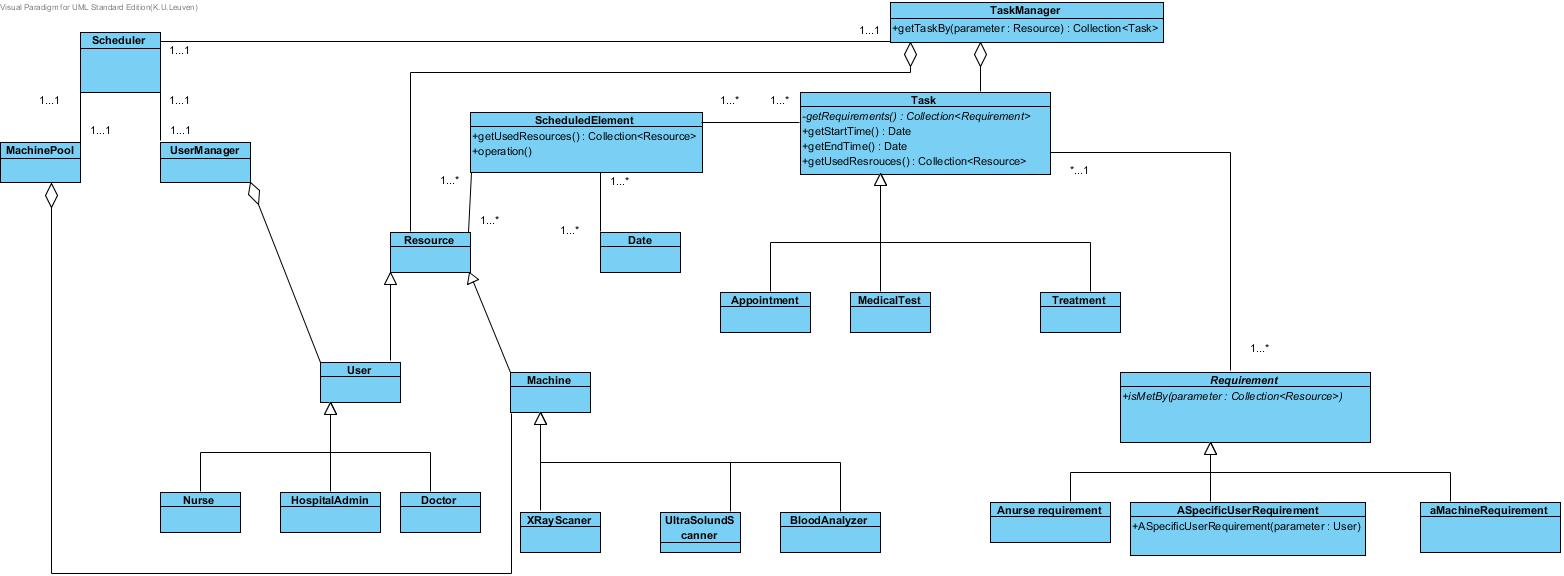
\includegraphics[width=200mm, height=120mm, angle=90]{schedulerfail0.jpg}
\section{Appendix II - Class diagram of the second revision of the scheduling system}
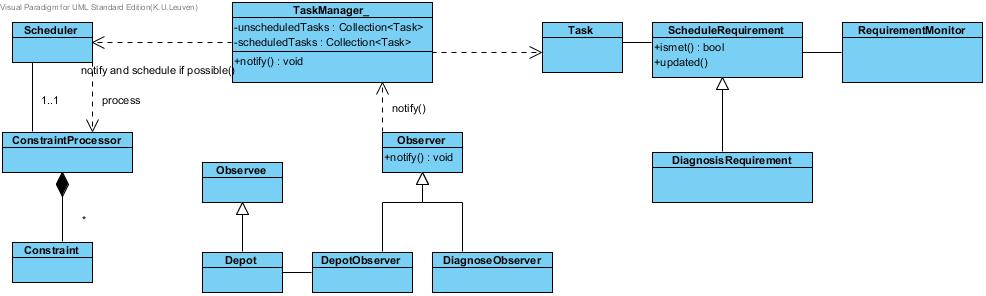
\includegraphics[width=200mm, height=70mm, angle=90]{schedulerfail1.jpg}
\section{Appendix III - Class diagram of the third revision of the scheduling system}
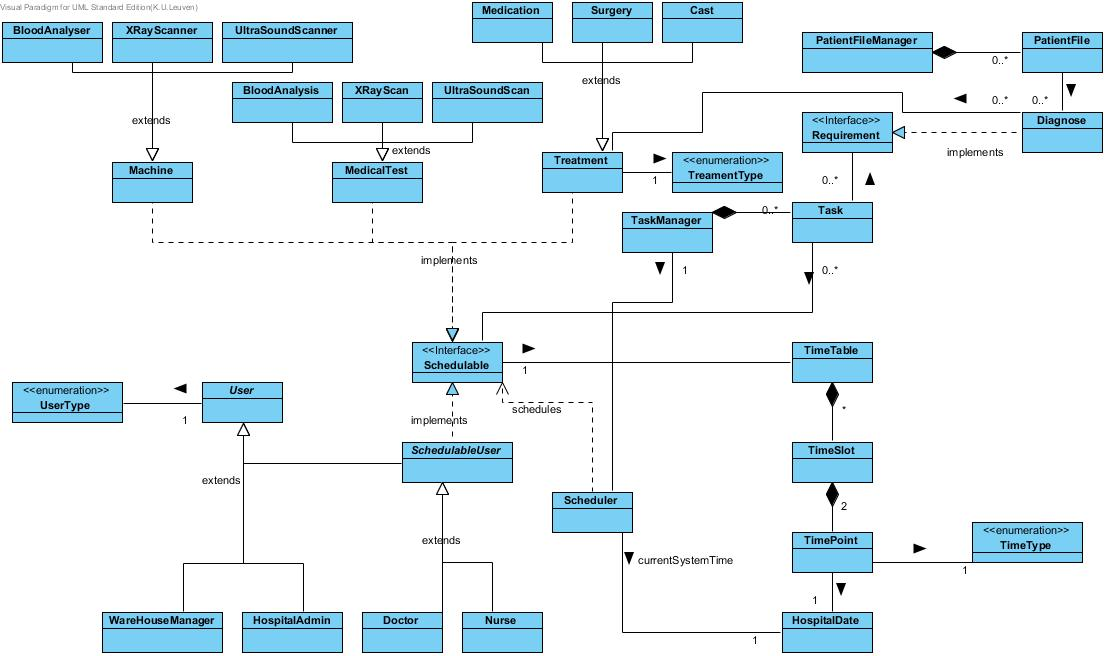
\includegraphics[width=200mm, height=170mm, angle=90]{schedulerwin.jpg}

\end{document}